\section{Choix du plan de jointure dans Asteroid}\label{sec:valid:perfs:couplage}
En section~\ref{sec:contrib:asteroid:reecriture:join}, nous avons présenté un opérateur capable de faire une jointure $\ssjoin$ entre une relation temporelle d'Astronef et une relation issue d'un SGBD. Deux plans ont été présenté : le plan \textbf{P1} applique la jointure dans Astronef en utilisant la relation temporelle issue du SGBD comme cache local ; le plan \textit{P2} quant à lui exécute l'opération de jointure à l'intérieur du SGBD pour exploiter ses capacités. Alors que l'optimisation poussant les opérateurs au plus proche du SGBD semble efficace dans la plupart des cas, nous voyons dans cette section que ce n'est pas toujours le cas pour cette opération.

\subsection{Jointure sur une relation statique}
Nous exécutons ici la requête $CPUMem$ présenté en section~\ref{sec:valid:domvision:requetes:historisation}. Pour rappel, cette requête implique une jointure avec $Application \Join Monitorable$ pour pouvoir identifier le flux de métriques processeurs et mémoires. Voici les paramètres d'expérimentations que nous fixons :
\begin{itemize}
	\item Les relations temporelles \textit{Monitorable} et \textit{Applications} sont considérées statiques
	\item La cardinalité d'\textit{Applications} est $N$
	\item La cardinalité de \textit{Devices} est $0.2N$ et celle de \textit{Monitorable} est de $1.2N$
	\item Il existe un index \textit{Application(monitorableId)}, \textit{Monitorable(monitorableId)} et sur \textit{Monitorable(name)}
	\item Il y a toujours suffisamment de mémoire pour exécuter les requêtes \textit{SQL}.
\end{itemize}

La requête \textit{SQL} automatiquement généré et donnée aux composants \textit{dbjoin} et \textit{dbsource} est la suivante :
\begin{lstlisting}[language=SQL]
SELECT deviceId as monitorableId, name 
FROM Application NATURAL JOIN Monitorable
\end{lstlisting}

\begin{figure}[ht]
	\centering
	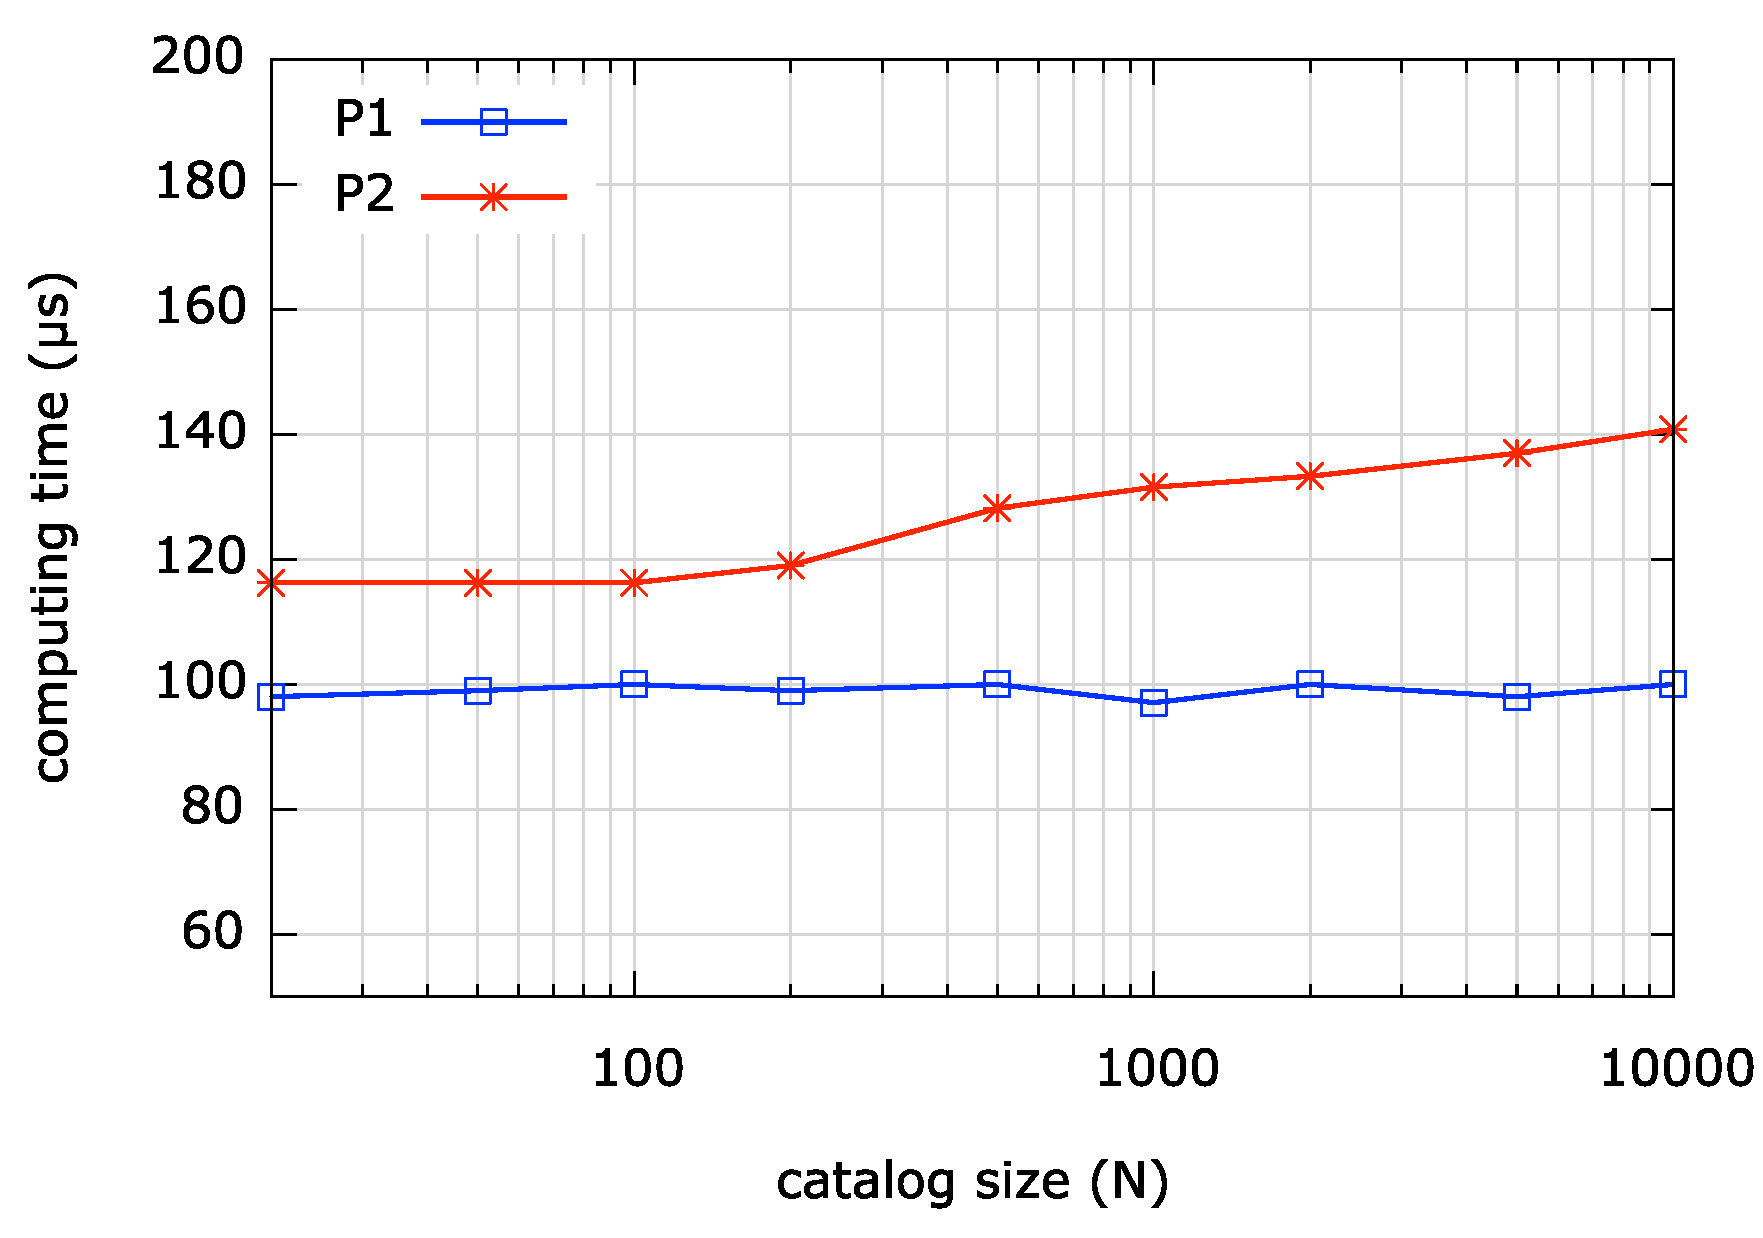
\includegraphics[width=0.66\textwidth]{valid-perfs-asteroid-static}
	\caption{Performance d'une jointure sur catalogue statique}\label{fig:valid:perfs:asteroid:static}
\end{figure}

\textbf{Résultats} : La figure~\ref{fig:valid:perfs:asteroid:static} montre la latence des deux plans de requête \textbf{P1} et \textbf{P2}. Les expérimentations ont montré que le plan \textit{P1} est meilleur et plus stable sur $N$. Bien entendu, cela ne pourra pas être le cas pour des valeurs très larges de $N$. Dans notre cadre expérimental, le \textit{hash-join} ne semble pas être le facteur limitant à $100\mu s$, car cela consiste à interroger une table de hachage constituée une seule fois. Le coût du \textit{scheduling} et d'autres tâches de l'intergiciel deviennent des facteurs limitants. 

Le plan \textbf{P2} est plus coûteux car pour chaque n-uplet, le composant doit se connecter au SGBD et exécuter la requête. Bien que la requête soit préparé, cela introduit un coût supplémentaire. Ce plan utilise l'index stocké sur disque dur, mais ses performances sont moindre comparé à un accès direct à une table de hachage en mémoire.

Si les relations \textit{Monitorable} ou \textit{Applications} sont mis à jour, cela introduit un surcout pour recalculer la table de hachage. Toutefois, le coût est absorbé au fur et à mesure du temps si les relations sont mises à jour rarement. Ainsi, le choix de \textbf{P1} est le meilleur pour la jointure avec des relations stables.

\subsection{Jointure sur un agrégat historique}
Dans cette seconde expérimentation, nous exécutons la requête $HistAvgCPU$ vu dans la section~\ref{sec:valid:domvision:requetes:alerte}. Pour rappel, cette requête joint une relation temporelle avec un agrégat effectué sur historique. Voici les paramètres de notre expérience :
\begin{itemize}
	\item L'historique est mise à jour dès que possible par un processus de collecte extérieur ($CPUMem$ par exemple).
	\item Il existe $D$ identifiants d'équipement et $M$ valeurs historique par identifiants.
	\item Il y a un index sur \textit{HistCPU(monitorableId)}.
\end{itemize}

La requête \textit{SQL} générée et donnée en paramètre à \textit{dbjoin} et \textit{dbsource} est la suivante : 
\begin{lstlisting}
SELECT monitorableId, AVG(cpu) as avg FROM HistCPU GROUP BY monitorableId
\end{lstlisting}

\begin{figure}[ht]
\subfigure[Performance globale]{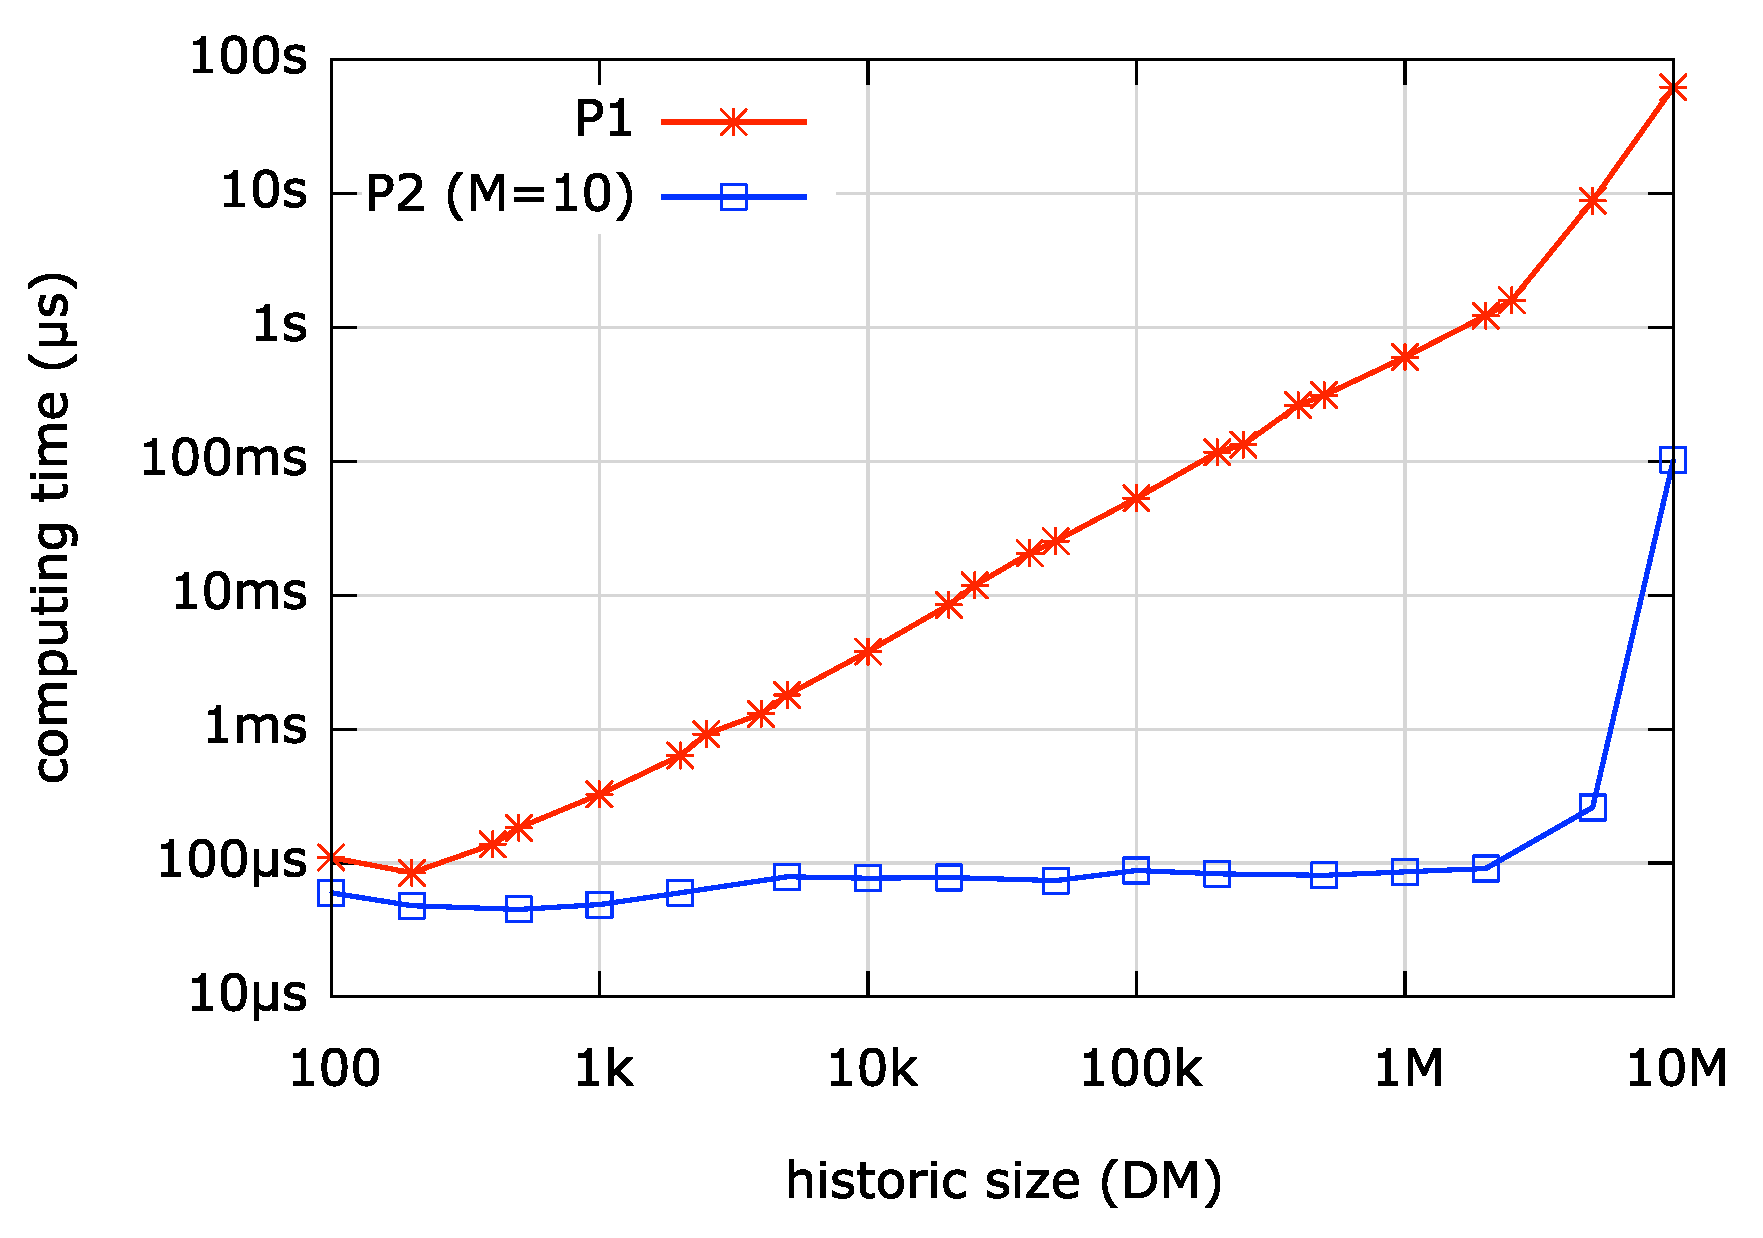
\includegraphics[width=0.48\linewidth]{valid-perfs-asteroid-aggregate}\label{fig:valid:perfs:asteroid:aggregate}}
\subfigure[Performance de l'agrégat avec sélection sur identifiant]{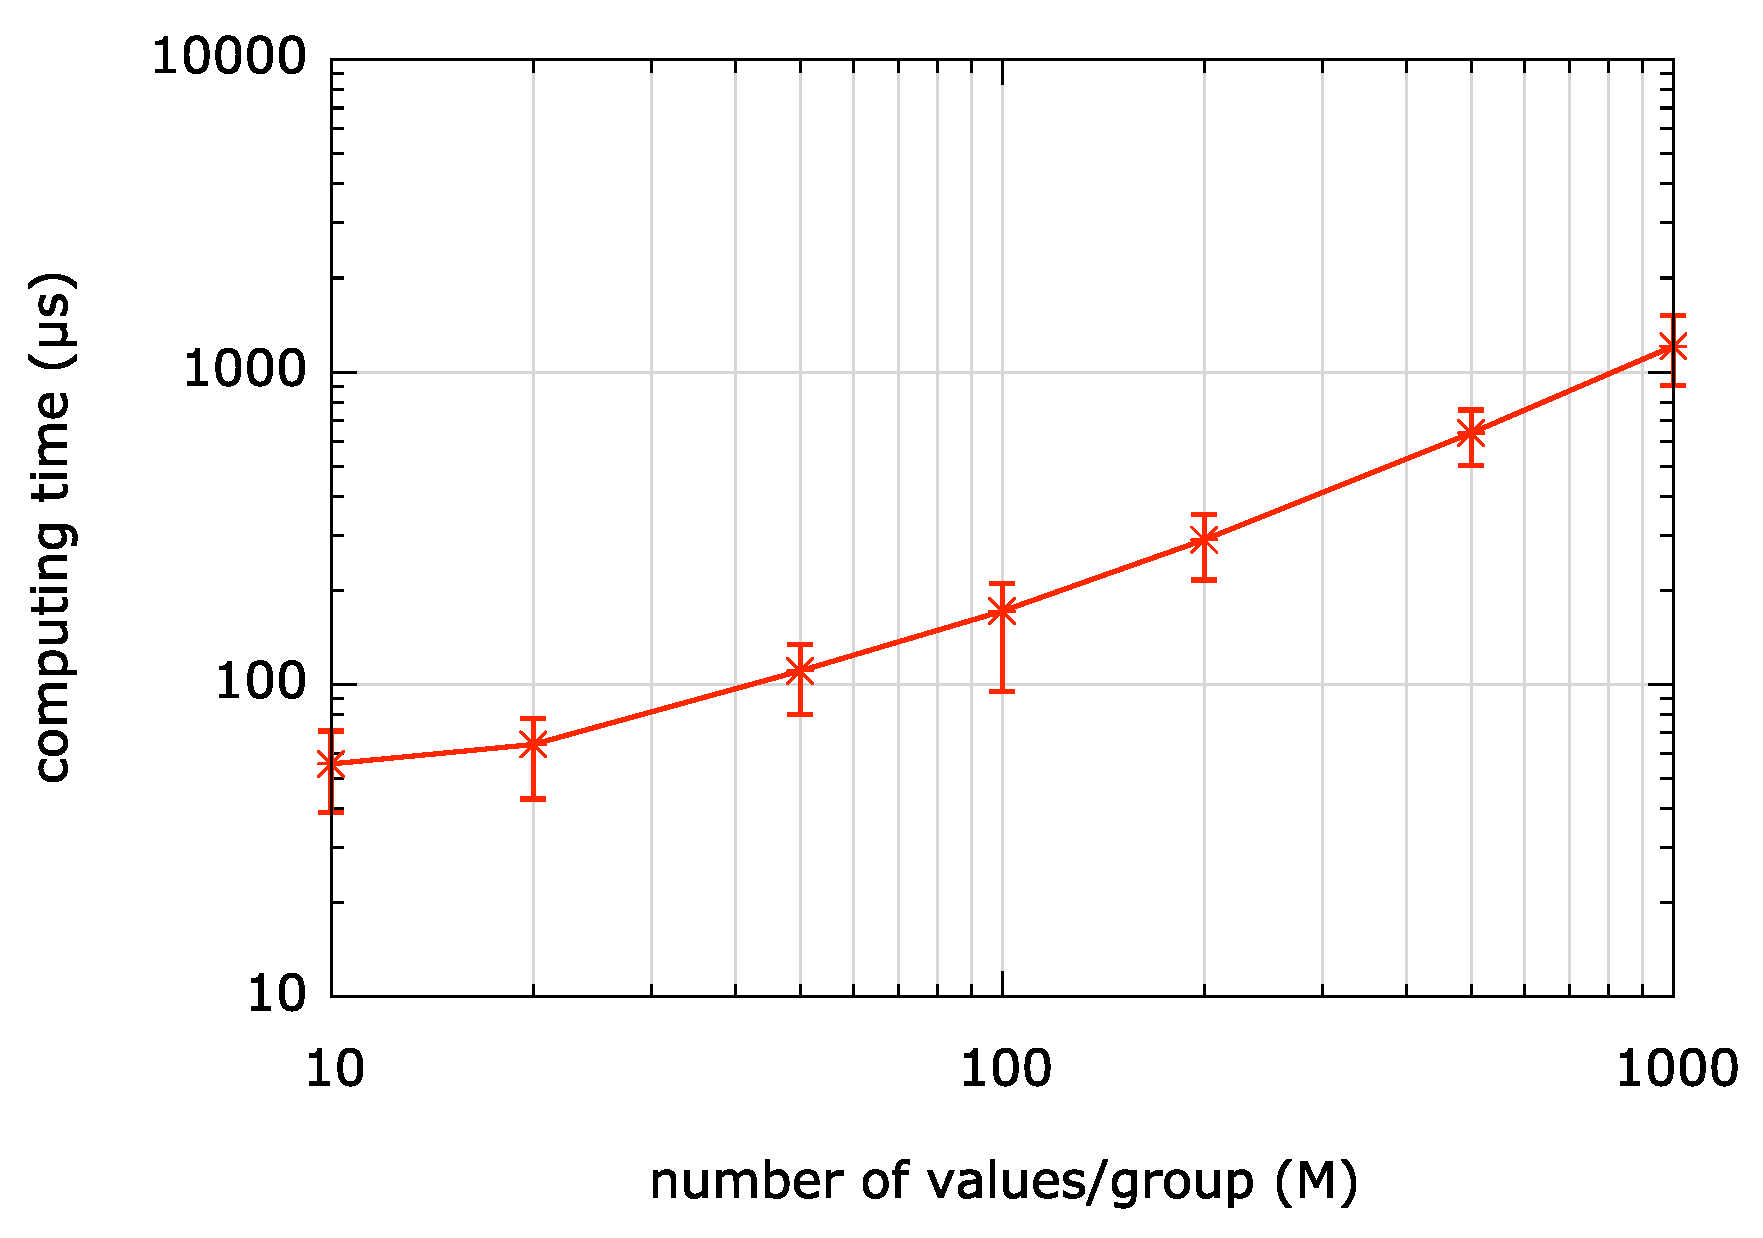
\includegraphics[width=0.48\linewidth]{valid-perfs-asteroid-aggregate-select}\label{fig:valid:perfs:asteroid:aggregate:select}}
\caption{Performance de la jointure avec agrégat en utilisant la sélection ou non}\label{fig:valid:perfs:asteroid:agg}
\end{figure}

\textbf{Résultats} : Dans cette expérience, nous avons pu remarquer que les performances de la requête \textit{SQL} de \textit{dbsource} ne dépend que de la taille de l'historique $(M.D)$. Toutefois, ce n'est pas le cas pour un agrégat utilisant une sélection sur l'identifiant avec \textit{dbjoin}, qui ne dépend principalement que de $M$. La figure~\ref{fig:valid:perfs:asteroid:aggregate} représente l'évolution de la latence de la requête d'agrégat avec et sans la sélection\footnote{La perte de performance massive observée après $4M$ de n-uplets est due au \textit{buffering} qui ne peut être fait en mémoire et le disque est utilisé. Ce fait a été confirmé par les développeurs d'\textit{H2}.}. La figure~\ref{fig:valid:perfs:asteroid:aggregate:select} représente l'évolution de la latence en variant $M$ pour l'agrégat avec sélection.

La performance dépend des caractéristiques de l'historique. Plus nous avons un $M$ petit, plus nous avons une petite latence pour le plan \textbf{P2}. La latence de \textbf{P2} est bornée entre les deux courbes de la figure~\ref{fig:valid:perfs:asteroid:aggregate} comme le cas $M=10$ représente le minimum de latence et $D=1$ (équivalent à aucune sélection) est le pire cas. Le choix du plan est clairement en faveur du plan \textbf{P2} car son pire cas a des performances similaires à \textbf{P1}. Dans l'expérience précédente, nous avions supposé pouvoir absorbé le coût de mise à jour. Ce n'est pas le cas ici car l'historique est régulièrement mis à jour.

\subsubsection{D'autres stratégies}
Si le résultat de la requête peut être dégradé, il est possible d'utiliser \textit{dbsource} est mode périodique. Dans ce cas, nous pouvons évaluer la condition limite pour passer d'un plan à l'autre en regardant les coûts mesurés dans la figure~\ref{fig:valid:perfs:asteroid:agg}.

Nous pouvons toutefois trouver une autre réécriture exacte. Lorsque la requête est déployé, il est possible de faire une distinction entre le passé $(CPUMemHistory^{t_0})$ et le futur représenté par le flux $CPUMem$. En supposant que l'agrégat est séparable par les moyens décrit dans la section~\ref{sec:rw:sgfd:optim:fenetres}, alors nous pouvons séparer les calculs sur le passé et le futur. L'agrégat passé est un calcul instantané effectué par \textit{dbsource} est mode \textit{one-shot}. L'agrégat futur est calculé par les opérateurs $_{id}\G[\infty]$. Or, ces opérateurs peuvent être regroupés en un seul macro-bloc capable de calculer l'agrégat avec un coût mémoire borné.